\chapter{Caratterizzazione di Dati Misurati e Statistica Inferenziale}
Resi noti una serie di dati misurati, quello che si vuole andare a fare è trovare un modello statistico che mi permetta di avere un'approssimazione valida di tali dati. Ci sono varie tipologie di tecniche e di approcci. Per grandi quantità di dati si farà un utilizzo massiccio della \textbf{Statistica inferenziale}, che comprende tutta una serie di metodi che permettono di andare a stimare un modello quantò più opportuno possibile ai dati che si stanno andando ad analizzare

\section{Media, Mediana e Moda}
Dato un insieme di dati, si possono andare a valutare 3 valori principali (e scalari), che ci permettono di approssimare (in maniera grossolana), la nostra distribuzione di dati (rappresentabile, anche, mediante un istogrammma). I valori a cui si fa riferimento sono:
\begin{itemize}
    \item \textbf{Media}: Media statistica di tutti i valori che si sta andando a considerare. Se si ha un set di valoi \(X = (x_1,x_2,\dots,x_n)\), allora definiamo come media:
    \[
    \overline{X} = \frac{1}{n}\sum_{i=1}^{n}x_i
    \]
    La media, però, non tiene conto dell'asimmetria dei dati (skewness), quindi se ad esempio un sistema ha dei tempi di ripsosta sempre stabili, e poi, un singolo caso di tempo di risposta lungo, potrebbe avere la stessa media di un sistema che ha mediamente tempi di risposta più lunghi (molto sensibile ad eventuali comportamenti limite)
    \item \textbf{Mediana}: La mediana di un set di valori \(X = (x_1,x_2,\dots,x_n)\) è data dalla selezione del valore centrale del set di valori ordinati. Per capire, si ordina il set di valori \(X\) e poi si seleziona l'elemento presente in \(\left\lfloor\frac{n}{2}\right\rfloor\). Ciò però presenta un problema, se il numrero di valori è dispari allora io seleziono l'unica posizione centrale presente (es. Se ho 3 elementi seleziono 1), mentre se ho un valore pari devo trovare un modo con cui scegliere quale elemento considerare, pertanto, essendo due i valori centrali, se ne fa la media (es. se ho 4 elementi, farò la media del valore in posizione 1 ed in posizione 2). La mediana a differenza della media viene presa direttamente dai valori reali e non calcolata considerando tutti i valori, ciò gli permette di essere più resistente agli outlier e sopratutto a distribuzioni asimettriche (resistente alla skewness)
    
    \item \textbf{Moda}: La moda rappresenta il valore più probabile all'interno di una distribuzione (quello presentato più volte). Di conseguenza tiene conto del picco presente nell'istrogramma. Il problema della moda è che può non esistere (caso di distribuzioni uniformi), oppure può assumere più di un valore (immaginare una distribuzione bi-gaussiana). Nonostante le considerazioni precedenti, la media è totalmente immune agli outlier (vedo solo il più probabile), e mi permette di evitare anche le ambiguità di una particolare distribuzione
\end{itemize}

\begin{info}
Nella descrizione dei parametri precedenti si è parlato di asimettrie dei dati (skewness dei dati), tale valore per piccole quantità di campioni può essere approssimato con la formula:
\[
skewness = \frac{y_{max}}{y_{min}}
\]
Da tale formula comprendo che più il valore è alto e più i dati sono "asimettrici". Ma tale considerazione è più corretta quanto più è piccola la quantità di campioni che sto andando a considerare 
\end{info}


Un semplice criterio per decidere quale tipologia di metrica utilizzare è quella mostrata in figura [\ref{img:criterio-media-mediana}]

\begin{figure}[h]
\centering
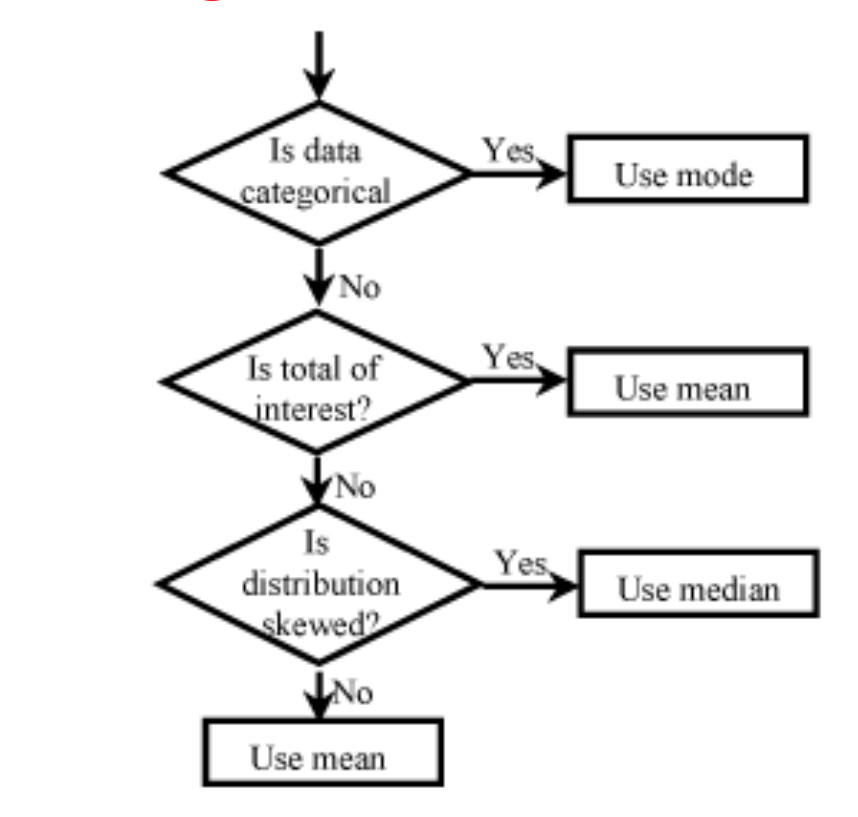
\includegraphics[width=.5\textwidth]{img/chapter-4/criterio-media-mediana.png}
\caption{Semplice schema di un criterio per la scelta della metrica da utilizzare}\label{img:criterio-media-mediana}
\end{figure}

I valori descritti, oltretutto, possono essere ottenuti osservando anche la distribuzione dei dati mediante degli istogrammi di occorrenza. In questo modo è anche più facile campire quale metrica sia meglio utilizzare.

\begin{figure}[H]
\centering
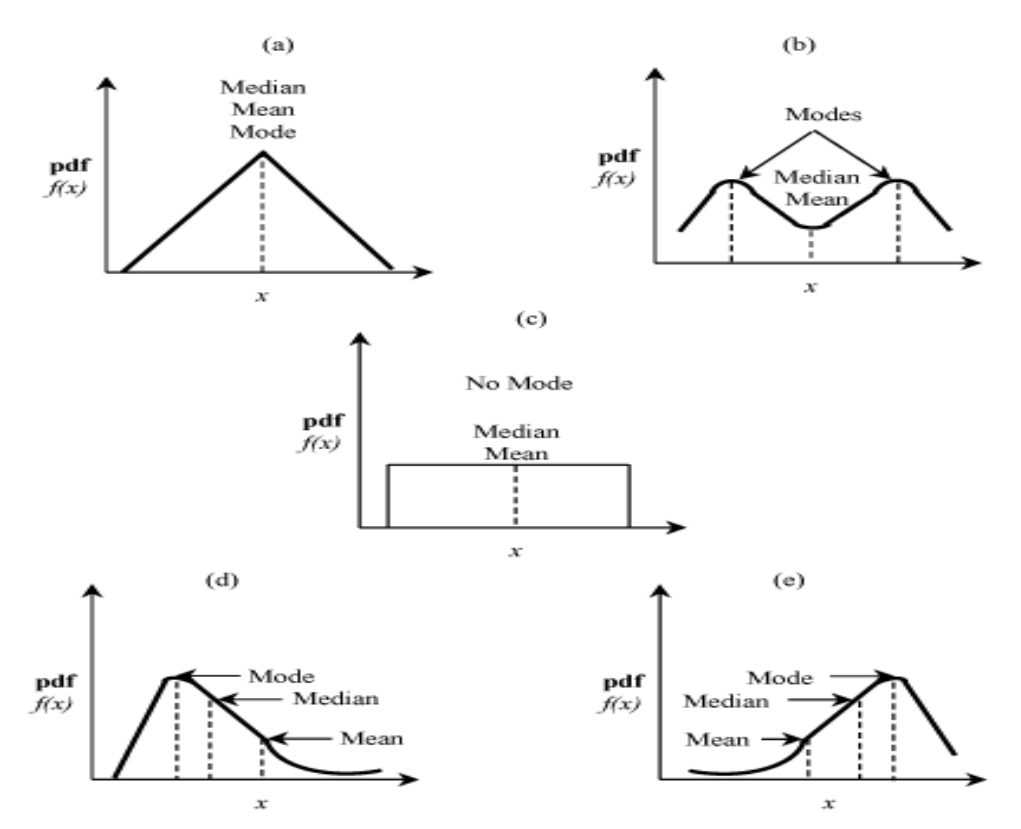
\includegraphics[width=.5\textwidth]{img/chapter-4/grafici-media-mediana.png}
\caption{Grafici illustrativi dei parametri discussi}\label{img:grafici-media-mediana}
\end{figure}

\section{Indici di dispersione}
Andare ad approssimare una distribuzione di valori con un singolo valore non basta, tale informazione non mi permette di considerare anche la \textbf{variabilità} che i dati possono avere nel tempo.
Uno strumento utile per avere un'idea della variabilità, sono gli \textbf{indici di dispersione}. Tra le metriche più utilizzate possiamo trovare:
\begin{itemize}
\item \textbf{Range}: Il range è un parametro molto basilare che viene calcolato come: \(v_{max} - V{min}\). Tale metrica, per quanto semplice, è anche molto poco resistente agli outlier
\item \textbf{Varianza campionaria (o deviazione standard)}: Tale parametro è strettamente calcolato dai dait e dipende dalla loro distribuzione
\item \textbf{10- e -90 Percentile}: Prendendo una distribuzione di dati si vanno a considerare due valori:
\begin{itemize}
    \item \textbf{\(P10\)}: Valore dei dati sotto il quale cade il 10\% dei dati considerati
    \item \textbf{\(P90\)}: Valore dei dati sotto il quale cade il 90\% dei dati considerati (quindi solo il restante 10\% è maggiore)
\end{itemize}
Si definisce poi come indice di dispersione il range calcolato su tali valori: \(range = P90-P10\). Se vediamo tali valori in riferimento alla pdf dei dati (il loro istogramma) e alla CDF. Si ha che per calcolare il valore P90 e P10, vado a valutare il valore della CDF in base al percentile ricercato (\(F(x_p) = 0.10\) o \(0.90\)), oppure, nel caso della pdf vado a calutare l'integrale (guardare la relazione tra CDF e pdf)\(\left [\int_{-\infty}^{x_p}f(x)dx = 0.10 | 0.90\right ]\). Il percentile solitamente può essere chiamato anche \textbf{quantile}. La differenza sta nella notazione, per il quantile si dice \(0.1\)-quantile (\(\alpha\)-quantile), mentre il percentile si esprime come 10-percentile (\(100*\alpha\)-percentile). Per stimare tali valori su un insieme di dati discreto (quindi non distribuzioni continue su cui effettuare integrali o derivate), posso andare ad effettuare, prima un ordinamento e poi a selezionare uno specifico valore in base alla \(\alpha\) scelta. Precisamente si va a selezionare il valore in posizione: \([(n-1)*\alpha + 1]\)

\item \textbf{Semi Inter-Quantile Range}: Tale metrica va ad utilizzare la definizione di due particolari casi di quantile. Più precisamente si va a considerare i quartili: \(0.75\)-quantile (75-percentile) [o terzo quantile] ed il \(0.25\)-quantile (25-percentile) [o primo quantile]. Tali valori sono poi combinati e si va a calcolare il valore del Semi Inter-Quantile Range come:
\[
SIQR = \frac{Q_3 - Q_1}{2}
\]

\item \textbf{Mean Absolute Deviation}: Vado a considerare la somma delle deviazioni, ma che sia sottoposta prima all'operazione di modulo, in modo da evitale l'azzeramento della somma delle deviazioni (come visto nel capitolo precedente). La formula è la seguente:
\[
MAD = \frac{1}{n}\sum_{i=1}^{n}|x_i - \overline{x}|
\]
Dove \(\overline{x}\) è la media dei valori: \(x_1,x_2, \dots, x_n\).

\end{itemize}

Un elemento utile quando si sta guardando il grafico dei dati è il \textbf{boxplot}. Il boxplot ci da un informazione grafica iniziale su dove i valori di interesse per il calcolo delle diverse metriche si trovino. Principalmente ci permette di poter osservare le seguenti metriche [\ref{img:boxplot}]:
\begin{itemize}
    \item \textbf{Valore massimo}
    \item \textbf{Valore minimo}
    \item \textbf{Mediana}(o 0.5-quantile/secondo quantile)
    \item \textbf{Primo Quantile}(0.25-quantile)
    \item \textbf{Terzo Quantile}(0.75-quantile)
    \item \textbf{Semi Inter-Quantile Range}
\end{itemize}

\begin{figure}[H]
\centering
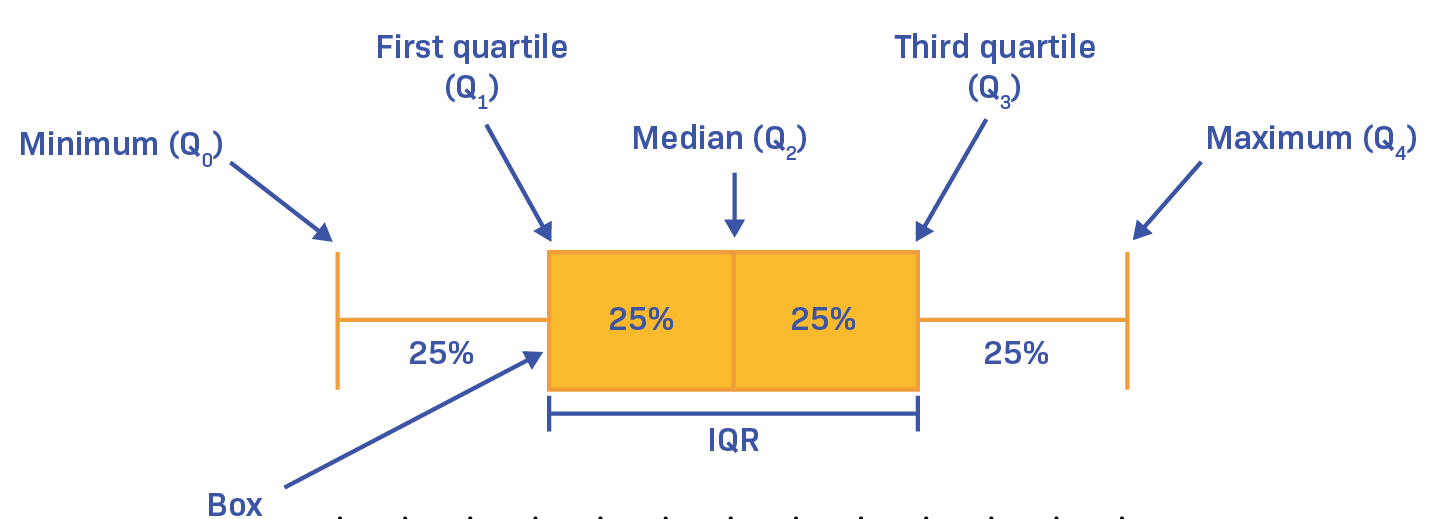
\includegraphics[width=.7\textwidth]{img/chapter-4/boxplot.png}
\caption{Struttura di un boxplot}\label{img:boxplot}
\end{figure}

La stima dell'indice di dispersione è qualcosa di complicato, sopratutto quando ci sono in mezzo gli outlier. Pertanto, solitamente, come metrica al posto della varianza (che non è completamente immune agli outlier), si preferisce utilizzare il Semi Iter-Quantile Range (SIRQ), che è più resistente alla presenza di outlier (anche più di qualcuno). Mentre come metrica centrale si preferisce l'uso della mediana, questo poichè ci è assicurato che esista (a differenza della moda), e sopratutto che faccia parte dell'insieme di valori considerato (diversamente dalla media). Questo spiega anche la costruzione del boxplot e dei valori che va a mettere in evidenza.

\section{Quantile-Quantile Plot}
Il \textbf{Quantile-Quantile Plot} è un metodo che ci permette di confrontare se due popolazioni hanno una distribuzione simile o meno. Nel nostro caso lo si utilizzerà per confrontare la distribuzione della nostra popolazione rispetto alla distribuzione normale.
La composizione di base di un grafico quantile-quantile generico è la seguente:
Si va a definire un punto \(p\) come \(p = (x_i, y_i)\), dove \(x_i\) è il valore teorico dell' i-esimo quantile, mentre \(y_i\) è il valore reale dell'i-esimo quantile. Per quanto riguarda i parametri reali non è complicato trovare i quartili (basta utilizzare la specifica formula in base ad \(\alpha\)), mentre per i parametri teorici risulta più complesso dato che bisogna trovare il modo di invertire la CDF. Per ricavare i valori della normale (funzione gaussiana di media nulla e varianza unitaria). Vado a calcolare il quantile come: \(q_i = \frac{i-0.5}{2}\), da cui posso ricavare il valore teorico come: \(x_i = 4.91\left [ q_i^{0.14} - (1-q_i)^{0.14} \right ]\).
Quindi, in generale, data una popolazione posso plottare il grafico utilizzando le metriche esposte in precedenza, e confrontare la distribuzione dei dati reali con quelli di una normale. In questo modo cerco di capire quanto la distribuzione della popolazione sia simile ad una distribuzione gaussiana. Alcuni esempi sono mostrati alla figura: [\ref{img:qqplot}]

\begin{figure}[h]

\centering
\begin{subfigure}[b]{0.5\textwidth}
\centering
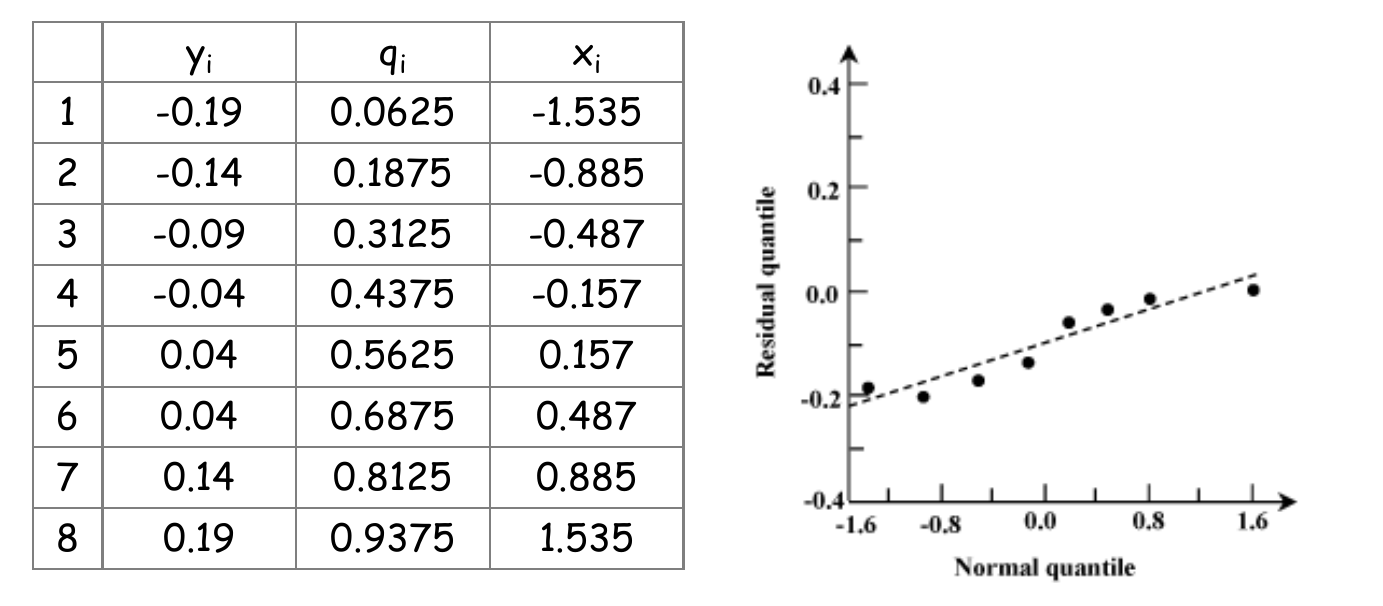
\includegraphics[width=\textwidth]{img/chapter-4/qqplot-ex.png}
\caption{Esempio di Quantile-Quantile plot rispetto alla normale}\label{img:qqplot-ex}
\end{subfigure}

\hfill

\begin{subfigure}[b]{0.6\textwidth}
\centering
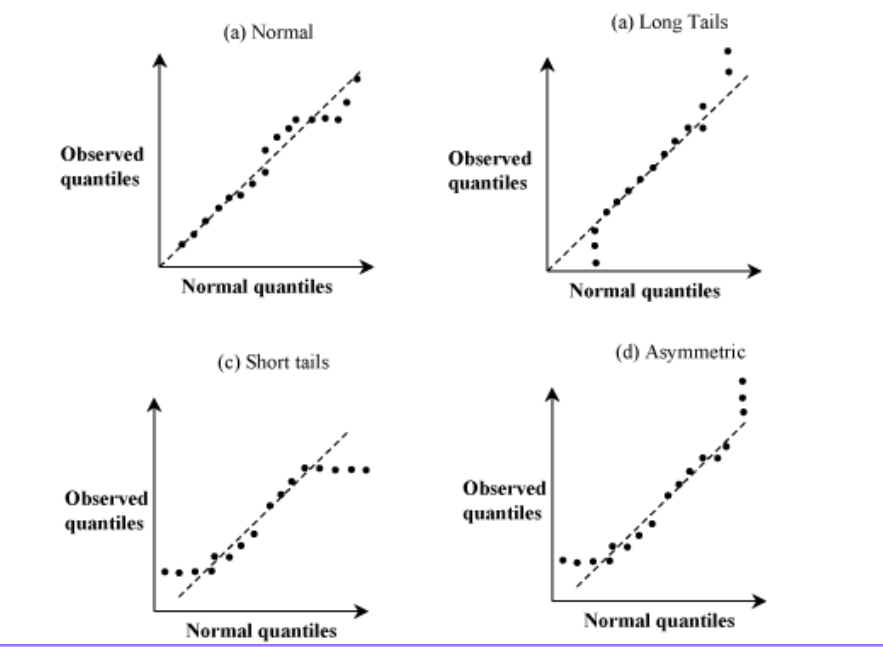
\includegraphics[width=\textwidth]{img/chapter-4/qqplot-confronto.png}
\caption{Diverse tipologie di rappresentazioni in base alla natura della popolazione}\label{img:qqplot-confronto}
\end{subfigure}

\caption{Applicazioni della Quanitile-Quantile plot (o  rappresentazione Quantile-Quantile)}\label{img:qqplot}
\end{figure}

\section{Intervalli di confidenza e dimensione del campionamento}
Solitamente, andare a considerare tutta la popolazione, potrebbe essere oneroso, pertanto, si potrebbe considerare di fare delle valutazioni su un numero minore di componenti estratte in maniera randomica (campionamento della popolazione). La problematica principale risiede nelle assunzioni che si potrebbe fare sulle statistiche della popolazione intera, ovvero, calcolare qualche valore per l'intera popolazione a partire dalla popolazione intera. Tali metodoligie sono sotto il nome di \textbf{statistica inferenziale}.
Per comprenderne bene il legame osservare l'immagine [\ref{img:statistica-inferenziale}].

\begin{figure}[h]
\centering
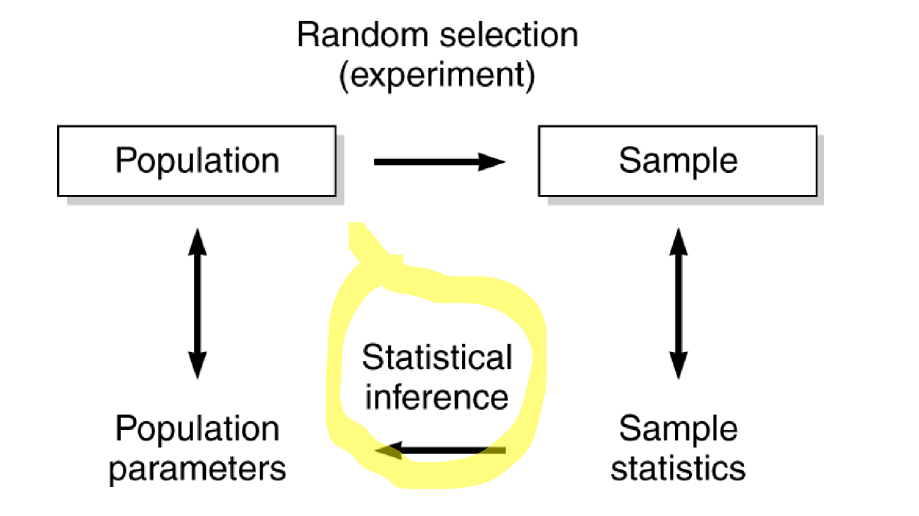
\includegraphics[width=.7\textwidth]{img/chapter-4/statistical-inference.png}
\caption{Collocazione logica della statistica inferenziale}\label{img:statistica-inferenziale}
\end{figure}

\subsection{Campioni e Popolazione}
\uppercase{è} importante definire cosa si intende quando si sta parlando di popolazione o di campioni, ciò ci permetterà di poter definire tutta una serie di principi statistici, utili, per effettuare l'inferenza statistica.
Formalmente si definisce \textbf{popolazione} l'insieme totale di tutte le componenti (o istanze), mentre si definisce \textbf{Campione}(O Sample), un insieme di n osservazioni provenienti dai campioni. In generale è importante, definire anche il significato di \textbf{parametri}, i dati associati alla popolazione, essi saranno indicati con le lettere greche (ad esempio la media e la varianza associate alla popolazione, tali valori per qualunque saranno i campioni estratti, non varieranno [saranno costanti]); mentre si definiscono \textbf{statistiche} i valori associati ai sample della popolazione, esse saranno rappresentate da lettere comuni (tali valori variano da campione a campione e quindi non sono costanti).

\clearpage
\begin{info}\label{inf:distribuzioni-Campionarie}
\textit{Tale pezzo non è richiesto ai fini dell'esame ma potrebbe essere utile in una fase di approfondimento e studio della statistica inferenziale}
    \\
\textbf{Distribuzioni Campionarie}\\
Si definisce \textbf{Distribuzione Campionaria}, una distribuzione di probabilità associata alla variabile aleatoria \(\overline{X}\), che è la composizione di diverse osservazioni \(X_1, X_2, \dots, X_n\) che sono ricavate da k-campioni della popolazione iniziale. \(\overline{X}\) non è altro che una variabile aleatoria associata alla media delle osservazioni (media campionaria).
\begin{warn}
Quando parliamo di \(\overline{X}\) stiamo parlando della variabile aleatoria (quindi un valore casuale), mentre la distribuzione campionaria è la funzione di distribuzione di probabilità(pdf) associata ad \(\overline{X}\)
\end{warn}

Pertanto, possiamo definire \(\overline{X}\) come:
\[
\overline{X} = \frac{X_1 + X_2 + \dots + X_n}{n}
\]
Da cui, applicando il \textbf{teorema fondamentale della media}, si ottiene che:
\[
E(\overline{X}) = \frac{E(X_1) + E(X_2) + \dots + E(X_n)}{n}
\]
Andando a considerare un caso più semplice, dove la popolazione ha media nota e pari a \(\mu\) e varianza \(\sigma^2\), e dove le variabili aleatorie \(X_1, X_2, \dots, X_n\), associate alle osservazioni dei campioni, sono delle variabili aleatorie indipendenti ed identicamente distribuite (sono la stessa variabile aleatoria con media \(\mu\) e varianza \(\sigma^2\), allora si può dire che:
\[
E(\overline{X} = \frac{\mu + \mu + \dots + \mu}{n} = \mu)
\]
\[
V(\overline{X}) = E((\overline{X} - \mu)^2) = \frac{\sigma^2 + \sigma^2 + \dots + \sigma^2}{n^2} = \frac{\sigma^2}{n}
\]
Da tali formule si sono ricavati dei valori associati alla distribuzione campionaria, dette statistiche. Com'è possibile notare, più la dimensione del sample size cresce e più la varianza diminuisce, ciò ci fa capire che l'errore fatto sulla media diminuisce man mano (base per la valutazione dello standard error).
Andando ad invalidare le ipotesi fatte sulla struttura della popolazione (sulla sua distribuzione di probabilità), allora si può andare a valutare il \textbf{Teorema del limite centrale}.
\end{info}

\subsection{Standard Error}
In linea generale e formale, lo \textbf{Standard Error} non è altro che la deviazione standard della distribuzione campionaria.
Quando vado a valutare le statistiche riferite ai vari campioni presi dalla popolazione, con sample size pari ad n, voglio capire quanto queste siano effettivamente vicine a quelle reali. La problematica risiede proprio nel calcolo dei parametri. Di base, non si possono fare delle assunzioni sulla distribuzione di probabilità della popolazione (solitamente non è gaussiana, ma ha una forma generica o skewed (ambigua)). Pertanto non posso andare a valutare la varianza campionaria, questo poichè non posso fare assunzioni. Pertanto, in questi casi, ci viene in aiuto il \textbf{teorema del limite centrale}.
Il \textbf{teorema del limite centrale} ci dice che:
\\\textbf{Ipotesi}\\
Siano \(X_1, X_2, \dots, X_n\), n-variabili aleatorie Indipendenti ed identicamente distribuite (hanno tutte la stessa distribuzione, poichè la loro base dei dati è la stessa)
\\
Sia la sample size n, un valore orientativamente grande \(n>=30\)
\\
\textbf{Tesi}
\\
Allora posso dire che la \textbf{distribuzione campionaria} della media (distribuzione della variabile aleatori \(\overline{X}\)), è riconducibile ad una funzione normale con:
\begin{itemize}
    \item \textbf{Media} pari a \(\mu\) (media della popolazione)
    \item \textbf{Varianza} pari a \(\frac{\sigma^2}{n}\) (o deviazione standard \(\frac{\sigma}{\sqrt n}\))
\end{itemize}
Se la sample size è relativamente bassa (empiricamente minore di 30), la distribuzione ha un'andamento differente chiamato \textbf{t-student}. (Questo accade poichè, solitamente, non conoscendo la varianza reale della distribuzione globale, si potrebbe andare ad utilizzare la varianza campionaria, ma tale varianza avrà anche lei un margine di errore [è una variabile aleatoria a n-1 gradi di libertà]. Di conseguenza quella relazione diventa una relazione assimilabile alla t-student).

\begin{info}
\textit{Tale pezzo non è richieto per lo svolgimento dell'esame, ma solo al fine di approfondire alcuni concetti}
\\
Seguendo quello che si è visto nel precedente approfondimento [\ref{inf:distribuzioni-Campionarie}]; Il teorema del limite centrale non è altro che la conseguenza della composizione della variabile aleatoria \(\overline{X}\), rispetto alle variabili aleatorie associate ai campioni. Se le variabili aleatorie sono indipendenti (ce lo assicurano le indipendenze tra le varie osservazioni) ed identicamente distribuite (il fatto che le varie variabili abbiano la stessa pdf(e quindi non lo stesso valore), ci assicura, che la  media di tutte le distribuzioni sia \(\mu\)), allora il teorema del limite centrale non è altro che la dimostrazione del caso particolare che si è mostrato in precedenza. Se si vuole avere una maggior formalità nell'esporre il teorema del limite centrale si può andare a definire, una nuova variabile aleatoria \(Z\), come:
\[
Z = \frac{\overline{X} - \mu}{\sigma / \sqrt{n}} 
\xrightarrow{\,n \to \infty\,} 
\mathcal{N}(0,1)
\]
Tale Z, solitamente, viene assimilata ad una \textbf{t-student}, poichè non è sempre detto che si conosca la \(\sigma\) reale associata alla popolazione, pertanto si va ad utilizzare la varianza campionaria \(s\). Data questa "sostituzione", come per la media, anche per la varianza bisognerebbe andare a definire degli intervalli di confidenza e degli errori rispetto al valore reale (pertanto viene trattata come una variabile aleatoria chi-quadrata), ciò ci permette di dire che la variabile aleatoria sopracitata \(Z\), sia a tutti gli effetti una \textbf{t-student}.
\end{info}

Il \textbf{Teorema del limite centrale} non fa alcuna ipotesi sulla distribuzione della popolazione di partenza. Pertanto si mostra un esempio di applicazione mediante la figura [\ref{img:central-limit}]

\begin{figure}[h]
\centering
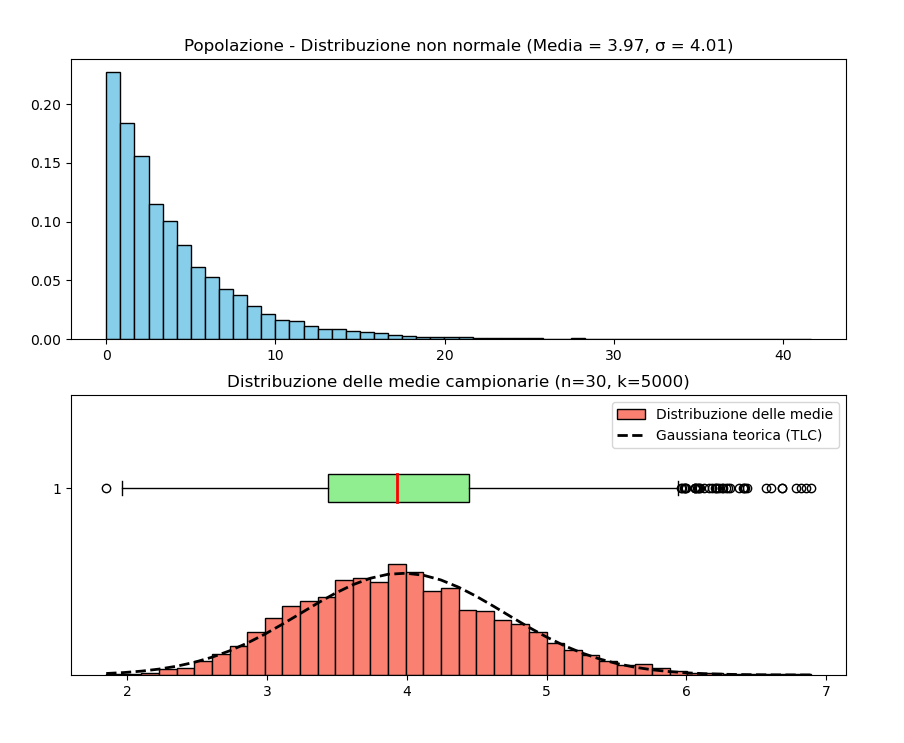
\includegraphics[width=.9\textwidth]{img/chapter-4/central-limit.png}
\caption{Applicazione del teorema del limite centrale}\label{img:central-limit}
\end{figure}

\subsection{Intervalli di confidenza}
Per comprendere appieno il significato di \textbf{intervallo di confidenza}, allora, bisogna esprimere in maniera migliore la variabile aleatoria \(\overline{X}\). Quello che si vuole andare a fare è normalizzarla, per cercare di ricondurre la distribuzione ad una normale con varianza unitaria. 
Formalmente potremo dire che:
\\
Siano \(X_1,X_2, \dots, X_n\) variabili aleatroie associate ai campioni di una popolazione che ha una distribuzione normale con una media non nota \(\mu\) ed una varianza nota \(\sigma^2\). Allora, la variabile aleatoria associata all'operazione di media \(\overline{X}\) è, teoricamente, normale, centrata in \(\mu\) e con varianza \(\sigma^2/n\). Pertanto, posso andare a normalizzare tale distribuzione di probabilità ad una normale standard mediante l'applicazione della seguente formula (simile allo z-score):
\[
Z = \frac{\overline{X} - \mu}{\sigma/\sqrt{n}}
\]

\begin{warn}
Per ora non si è ancora detto nulla sul come sia fatta la varianza, pertanto, se ci sono dei dubbi, risulta perfettamente in linea dato che ancora deve essere affrontata la questione. Essa sarà affrontata nel capitolo [\ref{par:iperparametri}]
\end{warn}

Un \textbf{Intervallo di confidenza}, quindi, non è altro che un intervallo numerico in cui la media ricade. In maniera formale, un intervallo di confidenza viene rappresentato mediante l'intervallo \([l,u]\), che ha la seguente caratteristica: \(l\leq\mu\leq u\). \(l\) e \(u\) sono valori che sono stati calcolati partendo dalle osservazioni che sono state campionate (quini i valori sono associati al singolo campione). Pertanto, dato che si andranno a valutare per ogni campione, costituiranno anche loro delle vere e proprie variabili aleatorie \(L\) ed \(U\). Supponendo di poterne valutare la distribuzione, si avrebbe che:
\[
P(L\leq \mu \leq U) = 1-\alpha
\]
dove \(0 \leq \alpha \leq 1\). Precisamente, l'intervallo delineato da \(l,u\) è l'intervallo di confidenza, mentre \(\alpha\) è il livello di confidenza (la probabilità che la media non faccia parte di tale intervallo). Dal singolo campione, quindi, possiamo ricavare che la media potrebbe ricadere all'interno dell'intevallo: \(l \leq \mu \leq u\). 

Per calcolare l'intervallo di confidenza a partire dai dati presenti, si va a considerare il valore che può assumere la precedente probabilità (\(1-\alpha\)), andando a fissare \(\alpha\), si possono andare a delimitare due punti simmetrici al punto della media della media campionaria, che delimitano due aree esterne la cui somma è proprio \(\alpha\) (di conseguenza due aree laterali che misurano \(\alpha/2\) l'una [\ref{img:gaussian-confidence}])

\begin{figure}[h]
\centering
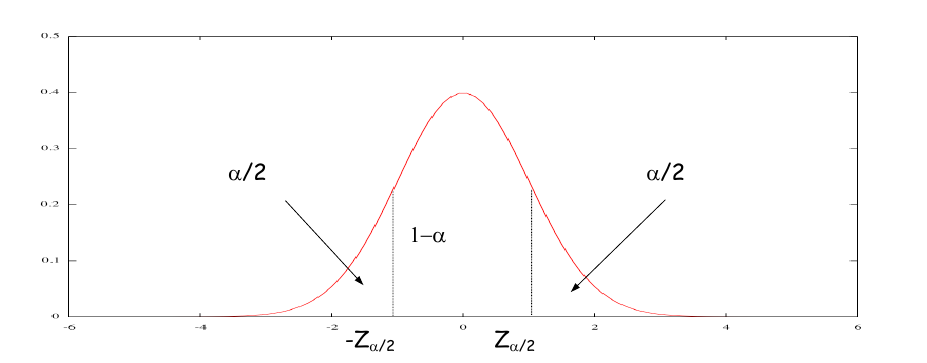
\includegraphics[width=.7\textwidth]{img/chapter-4/gaussain-confidence.png}
\caption{Intervallo di confidenza rispetto alla normale}\label{img:gaussian-confidence}
\end{figure}

Pertanto, essendo i valori della normale standard, noti, possiamo andare a scrivere la seguente probabilità:

\[
P(-z_{\alpha/2} \leq Z \leq z_{\alpha/2}) = 1 - \alpha
\]

Andando a sostituire con il valore che ci siamo calcolati a partire dalla variabile aleatoria associata alla distribuzione campionaria, si ha:
\[
P(-z_{\alpha/2} \leq \frac{\overline{X} - \mu}{\sigma/\sqrt{n}} \leq z_{\alpha/2}) = 1 - \alpha
\]

da cui:
\[
P\left (\overline{X} - z_{\alpha/2}\frac{\sigma}{\sqrt{n}} \leq \mu \leq \overline{X} + z_{\alpha/2}\frac{\sigma}{\sqrt{n}} \right ) = 1 - \alpha
\]
Da tale conclusione possiamo ricavare l'intervallo di confidenza (quindi i valori \(l\) e \(u\)).
Considerando quindi, \(\overline{x}\) la media della distribuzione campionaria, \(\sigma^2\) la varianza della popolazione iniziale (tale parametro non è banale) e sample size pari ad n, allora posso definire un \textbf{intervallo di confidenza} al \(100*(1-\alpha)\%\) di \textbf{livello di confidenza}, come: 

\[
\overline{x} - z_{\alpha/2}\frac{\sigma}{\sqrt{n}} \leq \mu \leq \overline{x} + z_{\alpha/2}\frac{\sigma}{\sqrt{n}}
\]
Con \(z_{\alpha/2}\) il punto di \(\frac{\alpha}{2}\)-quaritile o 100*(\(\frac{\alpha}{2}\))-percentile
\\
La lunghezza dell'intervallo di confidenza ci permette di misurare la \textbf{precisione} di stima, o meglio, ci dice il range in cui la media originale della popolazione possa ricadere con un certo livello di confidenza (solitamente 95\%, ma dipende dall \(\alpha\) utilizzata per in calcolo dell'intervallo).
Oltretutto, si può calcolare anche il margine di errore che si effettua con la media reale mediante la valutazione del seguente valore:
\[
E = error = |\overline{x} - \mu|
\]

\begin{warn}
Fare attenzione quando leggete tali appunti. \(\overline{X}\) il valore che ha X grande indica la variabile aleatoria a cui la distribuzione campionaria funge da pdf. Mentre \(\overline{x}\) è il valore della media calcolata per il singolo campione (o insieme di osservazione estratto dalla popolazione)
\end{warn}

I fattori che principalmente incidono sulle dimensioni dell'intervallo di confidenza sono:
\begin{itemize}
    \item \textbf{Sample size (n)}: Il sample size incide profondamente sulla dimensione dell'intervallo di confidenza. Più esso è grande e più il valore di media calcolato sul singolo campione risulta "preciso". (per intenderci, matematicamente, si va a ridurre il range a parità di livello di confidenza, in cui la media originale può ricadere)
    
    \item \textbf{Livello di confidenza}: Più il livello di confidenza è alto e più il range tende ad aumentare, mentre se si richiede dei livelli di confidenza più bassi, allora il range tende a diminuire. (si va ad agire, matematicamenre, sempre sul termine che va ad infierire sulla media nel calcolo del range. Per capirci, il livello di confidenza infierisce sul calcolo del parametro \(z_{\alpha/2}\))
    
    \item \textbf{Variabilità della popolazione}: Altro parametro fondamentale per il calcolo dell'intervallo di confidenza è la deviazione standard della popolazione iniziale, più la popolazione iniziale ha una deviazione standard grande, più è difficile dedurre la media a partire dai campioni

\end{itemize}

\subsection{Iperparametri per gli intervalli di confidenza}\label{par:iperparametri}
Nel precedente paragrafo si è affrontato la discussione riguardante gli intervalli di confidenza. Quello di cui però non si è discusso è il come gli iperparametri associati alla determinazione dell'intervallo di confidenza (\(n\),\(\sigma\)), vengano valutati o scelti. Pertanto, si sono definite delle regole, che ne hanno permesso la corretta valutazione.

\subsubsection{Sample size}
La \textbf{Sample size} è un parametro molto importante è va valutato con cura (date tutte le implicazioni che si hanno su di esso). Pertanto si è cercato un metodo di calcolo per valutarne al meglio il valore. 
Formalmente:

Definito \(\overline{x}\) il valore approssimativo (valutato sul singolo campione) della media \(\mu\) e \(\sigma\) la deviazione standard della popolazione e scelti: il livello di confidenza \(100*(1-\alpha)\%\) e la stima superiore dell'errore desiderato \(E\)(definito come \(E=|\overline{x} - \mu|\)). Allora si può calcolare la sample size come:
\[
n = \left ( \frac{\sigma * z_{\alpha/2}}{E} \right )^2
\]
Tale valore sarà un valore reale, dato che \(n\) dev'essere un'intero, allora si approssima sempre tale valore per eccesso, questo per garantire che i valori che sono stati dati in ingresso (\(E\), \(\alpha\)) siano rispettati.

\begin{info}
\textit{Tale pezzo è stato inserito sono a scopo di approfondimento, non è richiesto ai fini dell'esame}
\\
Il calcolo della \textbf{Sample size}, deriva direttamente dalla definizione di intervallo di confidenza, combinata con la definizione di errore. Precisamente la dimostrazione è composta dai seguenti passaggi:
Partendo dalla definizione dell'intervallo di confidenza:
\[
\overline{x} - z_{\alpha/2}\frac{\sigma}{\sqrt{n}} \leq \mu \leq \overline{x} + z_{\alpha/2}\frac{\sigma}{\sqrt{n}}
\]
Spostando la media al centro si ottiene:
\[
- z_{\alpha/2}\frac{\sigma}{\sqrt{n}} \leq \mu - \overline{x} \leq z_{\alpha/2}\frac{\sigma}{\sqrt{n}}
\]
Se al centro poniamo un modulo, otteniamo la definizione di \(E = |\overline{x} - \mu| = |\mu - \overline{x}|\), ma, essendo che i valori saranno sicuramente maggiori di 0 (dato l'inserimento del modulo), allora posso ignorare la parte di sinistra della disequazione, ottenendo:
\[
E \leq z_{\alpha/2}\frac{\sigma}{\sqrt{n}}
\]
Dato che cerchiamo il valore minimo, si può ignorare il minore e considerare solo l'uguaglianza, da cui:
\[
E = z_{\alpha/2}\frac{\sigma}{\sqrt{n}} \iff n = \left ( \frac{\sigma * z_{\alpha/2}}{E} \right )^2
\]
Da cui la tesi
\end{info}

\subsubsection{Varianza}
Fino ad ora abbiamo considerato la deviazione standard della popolazione \(\sigma\), nota. Solitamente, però, non si ha a che fare con popolazioni caratterizzate (non si conosce ne la media ne la varianza). Per risolvere tale problema si fa utilizzo del \textbf{Teorema del limite centrale}, che ci permette di dire che, date le variabili aleatorie (\(X_1,X_2,\dots,X_n\)) legate alla variabile aleatoria della media campionaria (\(\overline{X}\)), e dato un valore di \(n\) abbastanza grande, allora, scalando con lo z-score la \(\overline{X}\), otteniamo una distribuzione normale standard, più formalmente:
\[
\overline{X}' = \frac{\overline{X} - \mu}{\sigma/\sqrt{n}}
\]
dato che però \(\sigma\) non lo conosciamo, esso può essere sostituito con la deviazione standard campionaria, che per grandi valori di n risulta eguale alla deviazione standard normale. Formalmente si può dire che:
\[
\hat{\sigma}^2 = \frac{1}{n-1}\sum_{i=1}^{n}(x_i - \mu)^2 = \frac{n}{n-1}\left ( \frac{1}{n} \sum_{i=1}^{n}(x_i - \mu)^2\right )
\]

Dove, per \(n\) molto grande (idealmente \(n \to \infty\)) il termine \(\frac{n}{n-1} \to 1\), e che quindi ci permette di trovare una buona approssimazione della varianza per la varianza campionaria. Quindi, da ora in poi, per n sufficientemente grandi si potrà dire che \(s \approx \sigma\).
Da tale considerazione, quindi, si farà riferimento alla distribuzione \textbf{t-student}, che sarà definita come:
\[
Z = \frac{\overline{X} - \mu}{s/\sqrt{n}}
\]
Tale distribuzione, per valori grandi di \(n\) [per via del teorema del limite centrale] tende ad essere una distribuzione normale standard, il che ci permette di poter definire l'\textbf{intervallo di confidenza per grandi campioni}(large sample confidence interval), come:
\[
\overline{X} - \frac{s * z_{\alpha/2}}{\sqrt{n}} \leq \mu \leq \overline{X} + \frac{s * z_{\alpha/2}}{\sqrt{n}}
\]
il quale avrà un certo \textbf{livello di confidenza} di approssimativamente: \(100*(1-\alpha)\%\).

\subsection{t-student}
Come accennato precedentemente, mediante un'operazione di z-socre sulla variabile aleatoria \(\overline{X}\), e considerando la varianza \(\sigma \approx s\), allora si avrà una variabile aleatoria detta \textbf{t-student}. Essa viene caratterizzata da due principali parametri (solitamente), ovvero, il parametro \(\alpha\) ed i suoi gradi di libertà (nel nostro caso \(n-1\)). La variabile aleatoria \(T\) viene definita come:
\[
T = \frac{\overline{X} - \mu}{s/\sqrt{n}}
\]
data tale definizione, cambia anche la definizione dell'\textbf{intervallo di confidenza}. Precisamente, la definizione si basa sulla considerazione che si sta avendo a che fare con una t-student, e che i suoi valori sono tabulati secondo sia la variabile \(\alpha\) che rispetto ai suoi gradi di libertà \(n-1\). Infatti, formalmente:
\[
\overline{x} - \frac{t_{(1-\alpha/2),n-1} * s}{\sqrt{n}} \leq \mu \leq \overline{x} + \frac{t_{1-\alpha/2,n-1} * s}{\sqrt{n}}
\]
il livello di confidenza associato a tale intervallo è pari a \(100*(1-\alpha)\%\).

\clearpage
\section{Test di ipotesi}
Un \textbf{test di ipotesi} è una serie di tecniche utilizzate per decidere se un \textbf{ipotesi} fatta sui dati sia veritiera o meno. Con le conoscenze pregresse (delle precedenti sezioni), si possono affrontare tali test. Uno dei più semplici in quest'ambito è lo \textbf{zero mean test}, tale test va a verificare semplicemente se l'intervallo di confidenza calcolato include 0 o meno [\ref{img:zero-mean}].

\begin{figure}[h]
\centering
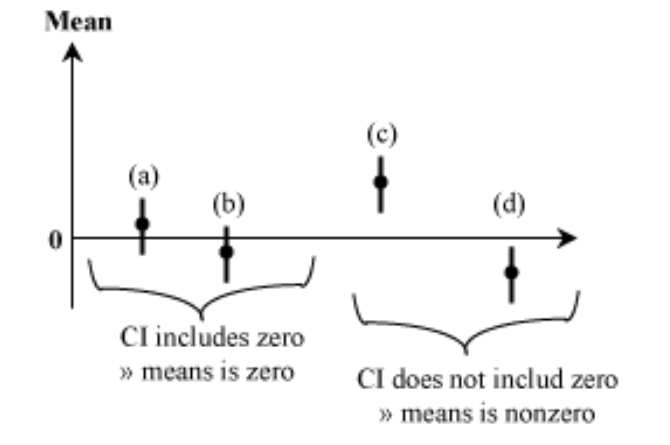
\includegraphics[width=.7\textwidth]{img/chapter-4/zero-mean.png}
\caption{Zero Mean Test}\label{img:zero-mean}
\end{figure}

I testi di ipotesi sono molto utili sopratutto quando si vogliono andare a confrontare diverse alternative (o diversi sistemi). Entrando nel merito, esistono due modalità principali con cui è possibile confrontare due diversi sistemi (A e B), ovvero;
\begin{itemize}
    \item \textbf{Paired observations}: Si vanno ad effettuare \(n\) esperimenti speculari su entrambi i sistemi, quindi entrambi avranno un set di espetimenti con cardinalità uguale. Pertanto si cerca di trovare una corrispondenza tra l'i-esimo test effettuato sul sistema A e l'i-esimo test effettuato sul sistema B.
    Una volta effettuati gli esperimenti si va a costruire la distribuzione delle differenze (\(d_i = A_i - B_i\)), e nel caso l'\textbf{intervallo di confidenza} include lo 0, allora i due sistemi sono statisticamente equivalenti.
    es. si hanno due sistemi e vengono sottoposti entrambi agli stessi 6 workload, voglio campire con un livello di confidenza del \(90\%\) se un sistema è "migliore" dell'altro. Una volta valutati i valori (magari del response time), vado a valutarne le varie differenze per coppie paired (vado ad effettuare la differenza tra valori appartenenti allo stesso workload), una volta ottenuto il vettore delle differenze vado a valutare l'intervallo di confidenza, se questo contiene 0 allora i due sistemi sono equivalenti atatisticamente, altrimenti sono statisticamente differenti.
    
    \item \textbf{Unpaired observations}: Si vanno ad effettuare le valutazioni su ogni sistema in maniera indipendente dall'altro (quindi non è detto siano gli stessi stress). Un volta ottenuti i risultati si vanno a costruire gli intervalli di confidenza, ognuno per se, e poi si può ricadere in tre casi:
    \begin{itemize}
        \item \textbf{Nessuma sovrapposizione}: I due intervalli di confidenza non si intersecano in alcun punto, il che predilige che un sistema sia prevalente all'altro
        \item \textbf{Medie incluse negli intervalli}: Quando i due intervalli di confidenza non solo si sovrappongono, ma la media dei due sistemi è inclusa nel range dell'altro e vicecersa (indice di equivalenza statistica)
        \item \textbf{Intervalli intersecati ma senza media}: Quando l'intersezione tra i due intervalli di confidenza è non nulla, ma le medie sono entrambe esterne all'altro intervallo di confidenza. In questi casi non è deducibile niente e bisogna effettuare un \textbf{t-test} (vedere [\ref{par:t-test}])
    \end{itemize}
    Per una migliore comprensione di quali di questi concetti osservare l'immagine [\ref{img:unpaired-observations}]
\end{itemize}

\begin{figure}[h]
\centering
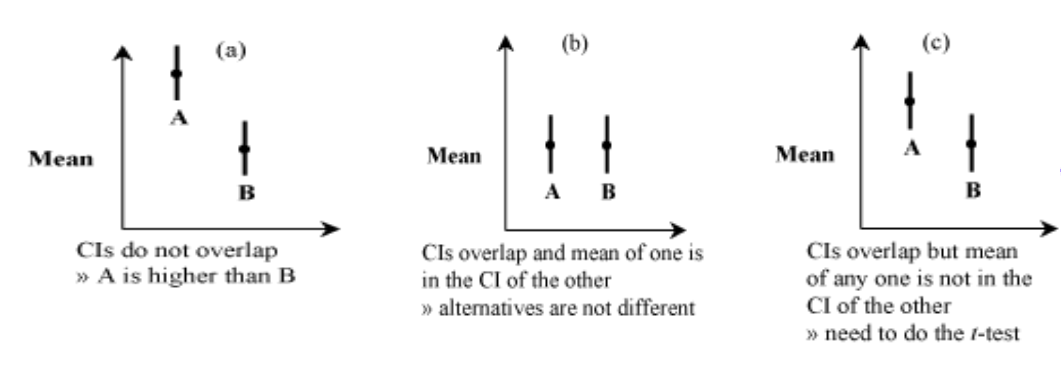
\includegraphics[width=.7\textwidth]{img/chapter-4/unpaired-observations.png}
\caption{Casi di unpaired observations}\label{img:unpaired-observations}
\end{figure}

Compreso cosa sia un \textbf{test di ipotesi}, allora, possiamo passare a definire quella che è un ipotesi:
\\
Un \textbf{ipotesi} non è che un affermazione che viene fatta sui parametri di una o più popolazioni. Ed il \textbf{test di ipotesi} non è altro che la procedura per confermare o meno le ipotesi. Si possono definire le ipotesi partendo dalla \textbf{Null Hypothesis}, essa racchiude quello che è il concetto che si vuole verificare (es. Ipotesi sulla media della popolazione \(H_0: \mu = \mu_0\)) [solitamente rappresenta lo stato corrente o quello senza effetto], e poi vi è la controparte detta \textbf{Alternative Hypothesis} [Afferma che c'è un effetto reale e solitamente quando si raccolgono i dati se cerca il modo di favorire \(H_1\) e di rigettare \(H_0\)]. Sulla alternative hypothesis si possono definire:
\begin{itemize}
    \item \textbf{one-sided alternative hyphotesis}: si va a definire una confutazione dell'ipotesi nulla evincendo una relazione d'ordine (es. \(H_1: \mu < \mu_0 \))
    \item La \textbf{two-sided alternative hypothesis}: si va a definire una confutazione dell'ipotesi nulla senza andare a mostrare particolari relazioni d'ordine (\(H_1:\mu \not = \mu_0\))
\end{itemize}

La suddivisione di tali ipotesi alternative risiede nel come poi si andranno a valutare le regioni critiche, principalmente, nella one-sided alternative hypothesis si va a definire la regione critica andando a valutare una sola delle code della gaussiana, mentre nel caso della two-sided alternative hypothesis si vanno a valutare entrambe le code della gaussiana (definite mediante quartili).

Fare dei test di ipotesi implica l’assunzione di decisioni che, in alcuni casi, possono risultare errate. Per questo motivo è fondamentale definire delle \textbf{metriche di valutazione del rischio}, in modo da quantificare e controllare la probabilità di giungere a una conclusione sbagliata. Nella pratica, raramente è possibile analizzare l’intera popolazione: si lavora quindi con campioni casuali, dai quali si ricavano informazioni utili per trarre conclusioni sulla popolazione di interesse. Attraverso l’\textbf{inferenza statistica}, si stima il comportamento dei parametri e si eseguono test di ipotesi per decidere se accettare o rifiutare l’ipotesi nulla \(H_0\) a favore dell’ipotesi alternativa \(H_1\). Tali procedure consentono di confrontare le formulazioni su basi oggettive, mantenendo sempre consapevolezza dei rischi associati e della probabilità di commettere errori nelle decisioni.

Per effettuare il \textbf{test di ipotesi}, solitamente, si effettuano i seguenti passi:
\begin{enumerate}
    \item \textbf{Dichiarazione dell'ipotesi nulla}: Effettuare un affermazione sui parametri della popolazione (ATTENZIONE non il campione ma la popolazione), ad es. (\(H_0: \mu = \mu_0\))
    \item \textbf{Livello di confidenza}: definizione di un parametro \(\alpha\) che indicherà la probabilità di commettere errori di \textbf{primo tipo}
    \item \textbf{Decidere la tipologia di test}: Scegliere quale test andare ad effettuare sui dati (es. t-test, z-test, ecc.)
    \item \textbf{Calcolo delle statistiche per il test}
    \item \textbf{Valutazione delle ipotesi}: la valutazione delle ipotesi differisce in base alla tipologia di test che si vuole andare ad effettuare
\end{enumerate}

\subsection{P-value}
Il \textbf{P-value approach} va a valutare il \textbf{p-value}, un valore che mi permette di capire quanto i miei dati siano compatibili con la mia ipotesi nulla. Per comprendere meglio il significato di tale valore facciamo l'esempio di una moneta:

\begin{info}
\textbf{\textit{Esempio moneta p-value}}\\
Si vuole valutare se una moneta sia equilibrata o meno. Pertanto si avranno le seguenti ipotesi:
\[
H_0: p(testa) = 0.5
\]
\[
H_1: p(testa) \not = 0.5
\]

Si effettuano 10 tiri e si ottiene testa 8 volte.
Allora si va a valutare il p-value come la probabilità che esca 8 volte testa \textbf{considerando l'ipotesi nulla come vera}. Pertanto si va a valutare che:
\[
P(testa\ per\ 9\ volte) = \binom{10}{8}\left (\frac{1}{2} \right )^8 * \left (\frac{1}{2} \right )^2 = 45\left (\frac{1}{2^10} \right ) = 0.04394 = 4.39\%
\]
Se ho considerato un livello di confidenza al \(90 \%\), il p-value, essendo minore del valore di \(alpha = 0.5\), allora l'ipotesi \(H_0\) è certamente falsa. Mentre nel caso fosse stato maggiore di tale valore, l'ipotesi \(H_1\) poteva essere confermata. Più è grande il p-value e maggiore è la "giusta" scelta dell'ipotesi \(H_0\)
\end{info}

In generale, la determinazione del p-value viene effettuata mediante l'integrale della distribuzione, che sottostà al valore effettivamente osservato (solitamente si lavora sui valori limite dell'ipotesi \(H_0\), quindi quei valori che sono al confine della scelta per tale ipotesi). 
Un'altro modo per interpretare il p-value è associandolo al \textbf{rischio} di un errato rigetto dell'ipotesi \(H_0\).

\subsection{Tipologie di errori}
Nel precedente capitolo si fa riferimento a \textbf{regione critica} e \textbf{valori critici}. Per capire meglio a cosa si fa riferimento, si va a considerare uno specifico intervallo di confidenza, in cui l'ipotesi \(H_0\) è vera. La \textbf{regione critica} è quella parte del dominio che rigetta l'ipotesi \(H_0\) mentre i \textbf{valori critici} sono i valori limite per la regione critica. La definizione di quali sia la regione critica ed i relativi valori critici viene definita a partire dalla tipologia di alternative hypothesis fatta, per comprendere al meglio cosa si intende per regione critica e per valori critici, osservare la figura [\ref{img:critical-regions}], dove le regioni in blu sono le regioni critiche, ed i valori evidenziati con delle linee nere, invece, sono i valori critici.

\begin{figure}[h]
\centering
\begin{subfigure}[b]{0.4\textwidth}
\centering
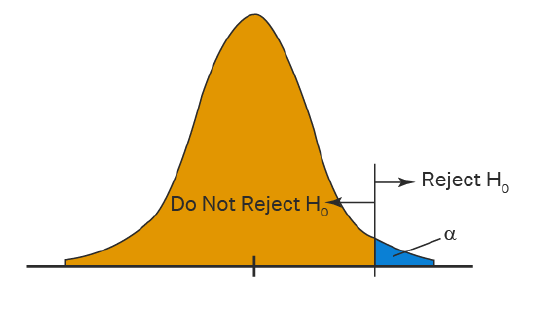
\includegraphics[width=\textwidth]{img/chapter-4/one-sided-critical.png}
\caption{One-Sided alternative hypothesis critical region}
\end{subfigure}

\hfill

\begin{subfigure}[b]{0.4\textwidth}
\centering
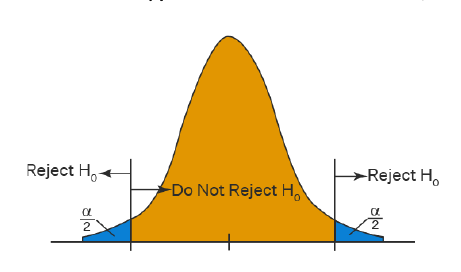
\includegraphics[width=\textwidth]{img/chapter-4/two-sided-critical.png}
\caption{Two-Sided alternative hypothesis critical regions}
\end{subfigure}

\begin{subfigure}[b]{0.5\textwidth}
\centering
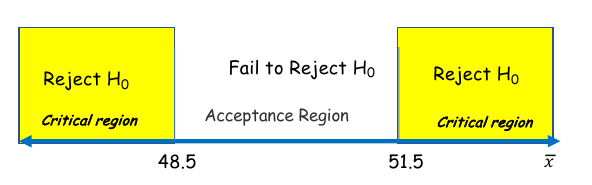
\includegraphics[width=\textwidth]{img/chapter-4/regioni critiche.png}
\caption{Two-Sided alternative hypothesis critical regions (esempio logico)}
\end{subfigure}

\caption{Critical region per le differenti tipologie di alternative hypothesis}\label{img:critical-regions}
\end{figure}

\subsubsection{Errore di tipo I}
L'\textbf{errore di tipo I} è definito come: Rigettare l'ipotesi nulla \(H_0\) quando essa è in realta vera. La probabilità associata all'errore di tipo I, viene chiamata \textbf{\(\alpha\)-error} (o significance level o dimensione del test. Sono varie le definizioni)
\[
\alpha = P(errore\ di\ tipo\ I) = P(H_0\ sia\ rigettato\ quando\ H_0\ e'\ vero)
\]
Per definire tale parametro si hanno due strade:
\begin{itemize}
    \item Decido il parametro \(\alpha\) e poi vado a valutarmi i valori critici e le regioni critiche
    \item La regione prefissata ed i valori critici sono stati fissati in precedenza, da tali valori vado a ricavarmi il mio parametro \(\alpha\)
\end{itemize}
Per comprendere al meglio come calcolare il parametro \(\alpha\) a partire dai valori critici, si fa il seguente esempio:
\\
Si considera un'intervallo di confidenza come [48.5, 51.5]. L'errore di tipo I occorre quando ho un valore di \(\overline{x}\) che è fuori dal range, quando nella realtà la media \(\mu=50\). Supponendo che la popolazione sia una gaussiana con media \(mu = 50\) e varianza \(\sigma^2 = 2.5^2\), andando a valutare la distribuzione delle medie campionarie, si ottiene una normale (per il teorema del limite centrale), con media \(\mu = 50\) e varianza \(\sigma^2 / n = \sigma/\sqrt{n} = 0.79\) = . Pertanto, si può andare a definire \(\alpha\) come:
\[
\alpha = P(\overline{X} < 48.5\ con\ \mu = 50) + P(\overline{X} > 51.5\ con\ \mu = 50)
\]
Andando a valutare gli z\_values, si ottiene:
\[
z_1 = \frac{lower\_critical\_value - \mu}{\sigma/\sqrt{n}} = \frac{48.5 - 50}{0.79} = -\frac{1.5}{0.79} \approx -1.90
\]
\[
z_2 = \frac{upper\_critical\_value - \mu}{\sigma/\sqrt{n}} = \frac{51.5 - 50}{0.79} = \frac{1.5}{0.79} \approx 1.90
\]

e quindi posso andare a definire \(\alpha\) come:
\[
\alpha = P(Z < -1.90) + P(Z > 1.90) \approx 0.028717 + 0.028717 = 0.057434
\]

Questo lo possiamo fare poichè mediante la "normalizzazione" della variabile aleatoria, possiamo accedere ai valori di probabilità andando a prelevarli all'interno delle tabelle inerenti alla funzione t-student.
Il valore trovato, ci permette di capire che rigettare l'ipotesi \(H_0: \mu=50\) quando la media è effettivamente \(\mu=50\) può accadere con una probabilità pari al \(5.74\%\).
La cosa da notare è che, se anche non cambiassi i valori critici, ma aumentassi la sample size, la probabilità di errore di tipo I diminuirebbe, il che aggiunge un ulteriore peso nella scelta della sample size effettiva.
Per capirci, aumenterebbe il valore associato alla varianza della distribuzione campionaria \(\sigma/\sqrt{n}\) Il che, indirettamente fa aumentare anche i valori delle \(z_1\) e \(z_2\), che aumentando in modulo, riducono l'area sottostante, e quindi la probabilità di avere un errore di tipo I
\[n = 16\]
\[\sigma/\sqrt{n} = 2.5/\sqrt{16} = 0.625\]
\\
\[z_1 = \frac{48.5 - 50}{0.625} = 2.4\]
\\
\[z_2 = \frac{51.5-50}{0.625} = 2.4\]
\\
\[\alpha = P(Z < 2.4) + P(Z > 2.4) = 0.0082 + 0.0082 = 0.0164 = 1.64\%\]
La probabilità di avere un errore di tipo I ora si è ridotta drasticamente, a parità di valori critici (con probabilmente un livello di confidenza diverso), ma ciò ci basta per capire come la sample size è importante anche per la definizione dell'errore di tipo I

\begin{figure}[h]
\centering
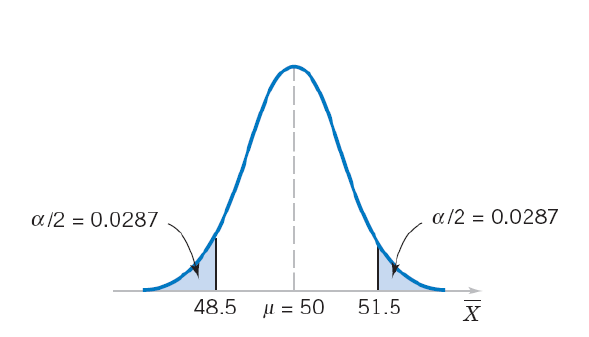
\includegraphics[width=.6\textwidth]{img/chapter-4/type_I_error.png}
\caption{Interpretazione grafica dell'errore di tipo I}\label{img:exercise-tipo-I}
\end{figure}

\subsubsection{Errore di tipo II}
L'\textbf{errore di tipo II} è definito come: Non Rigettare l'ipotesi nulla \(H_0\) quando essa è in realta falsa. La probabilità associata all'errore di tipo II, viene chiamata \textbf{\(\beta\)-error}.
\[
\beta = P(errore\ di\ tipo\ II) = P(Non\ rigetto\ di\ H_0\ quando\ H_0\ falso)
\]
Per comprendere in magliera ottimale la suddivisione tra le due tipologie di errori, si può far riferimento alla tabella [\ref{tab:error-types}]

\begin{figure}[h]
\centering
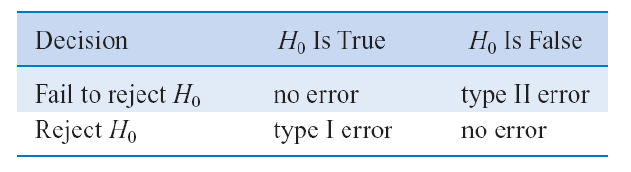
\includegraphics[width=.7\textwidth]{img/chapter-4/tabella-type-errors.png}
\caption{Tabella per comprendere la posizione e la definizione degli errori di tipo I e II}\label{tab:error-types}
\end{figure}

Per capire appieno come interpretare l'\textbf{errore di tipo II}, si va a svolgere il seguente esempio:
\\
Consideriamo sempre l'esempio precedente dove si ha l'intervallo di confidenza [48.5, 51.5], e la varianza della popolazione nota \(\sigma = 2.5\). 
Andare a valutare l'errore di tipo II vuol dire:
\[
\beta = P(errore\ di\ tipo\ II) = P(Non\ rigettare\ H_0\ quando\ H_0\ e'\ falsa)=
\]
\[
P(48.5 \leq \overline{X} \leq 51.5\ con\ \mu=52)
\]
andando a valutare i valori delle \(z_1\) e \(z_2\), si avrà:
\[
z_1 = \frac{lower\_critical\_value - \mu}{\sigma/\sqrt{n}} = \frac{48.5 - 52}{0.79} = -\frac{3.5}{0.79} \approx -4.43
\]
\[
z_2 = \frac{upper\_critical\_value - \mu}{\sigma/\sqrt{n}} = \frac{51.5 - 52}{0.79} = -\frac{0.5}{0.79} \approx -0.63
\]
da cui andando a sostituire mediante la variabile normalizzata, si avrà che:
\[
P(-4.43 \leq Z \leq -0.63) = P(Z \leq -0.63) - P(Z \leq -4.43) = 0.2643 - 0.0000 = 0.2643 = 26.43\%
\]
Tale percentuale è il valore di \(\beta\) che indica la probabilità di commettere l'errore di non rigettare l'ipotesi \(H_0\) a discapito del reale valore assunto dalla media.
Si vuole far notare che l'errore di tipo II aumenta quanto più diminuisce la distanza tra la media effettiva e quella che si vuole testare. Per capire, se prima la media reale fosse stata \(50.5\) al posto di \(52\), si sarebbe avuta la seguente probabilità di errore di tipo II:
\[
z_1 = \frac{48.5 - 50.5}{0.79} = -\frac{2}{0.79} \approx -2.53
\]
\[
z_2 = \frac{51.5 - 50.5}{0.79} = \frac{1}{0.79} \approx 1.27
\]
Valutando la probabilità tramite la formula scomposta della \(Z\):
\[
P(Z \leq 1.27) - P(Z \leq -2.53) = 0.8980 - 0.0057 = 0.8923 = 89.23\%
\]
Notiamo come con la riduzione della "distanza" tra le due medie, aumenta la probabilità di errore di tipo II. A livello grafico, viene rappresentato come l'area sottostante la distribuzione reale per cui si darebbe l'ipotesi sbagliata (compresa tra i valori critici). Per capire meglio tale concetto osservare la figura [\ref{img:type-II-error}].

\begin{figure}[h]
\centering
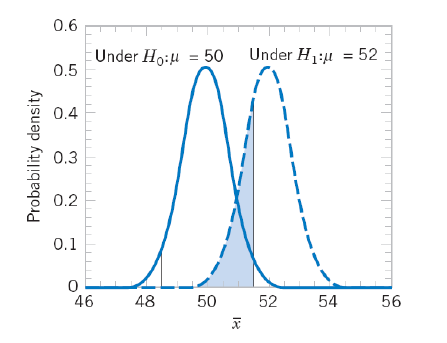
\includegraphics[width=.6\textwidth]{img/chapter-4/type-II-error.png}
\caption{Area a cui è associata la probabilità di tipo II (caso test per media 50 con media effettiva 52)}\label{img:type-II-error}
\end{figure}

Come anche per l'errore di tipo I, l'errore di tipo II è fortemente legato alla sample size, più essa è alta e più l'errore di tipo II diminuisce, questo poichè un aumento della sample size fa sì che aumenti anche il valore in modulo delle \(z_i\), che, più sono grandi e minore saranno le loro probabilità, di conseguenza, sarà minore anche l'errore di tipo II (\(\beta\)).

\subsection{Potenza di un test statistico}
Gli errori che si sono definiti in precedenza non bastano per definire quanto un test valuti correttamente le sue ipotesi. Pertanto di definisce la \textbf{potenza} di un test statistico, come la probabilità di rigettare l'ipotesi nulla \(H_0\) quando l'ipotesi alternativa è vera. (tale definizione viene data, dato che gli errori parlano di "falle" che il test può avere, il che ci fa capire che non ci sono abbastanza informazioni per avere la risposta corretta [con una certa probabilità], ma non si va a valutare, invece, quanto il test di ipotesi sia tollerante rispetto ad altre implicazioni). La potenza di un test statistico valuta ed esprime la \textbf{sensitività} del test statistico, dove per sensitività si intende l'abilità di un test di riconoscere le differenze. La definizione formale di tale parametro è:
\[
power = 1 - \beta
\]
che sta ad indicare la probabilità di rifiuto di un ipotesi \(H_0\) che è effettivamente falsa. A livello grafico corrisponde all'area sottesa alla curva originale (quella con l'ipotesi di media vera, che risiede al di fuori del critical value, che sta ad indicare quando l'ipotesi \(H_0\) viene rigettata per un motivo valido dato dalla distribuzione valida)[\ref{img:power-value}].

\begin{figure}[h]
\centering
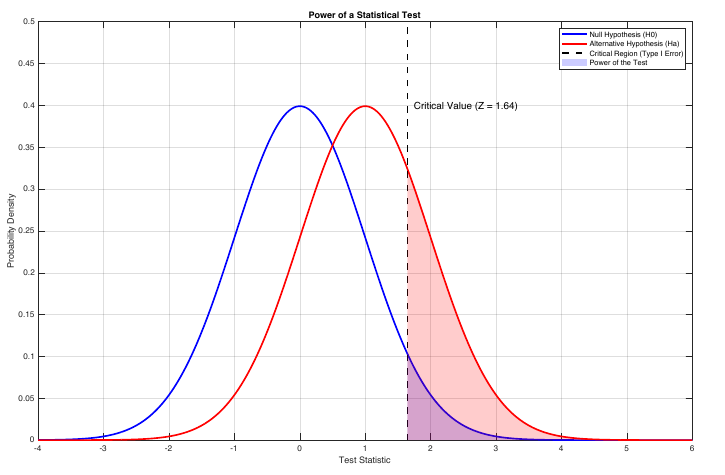
\includegraphics[width=.7\textwidth]{img/chapter-4/power-value.png}
\caption{Definizione grafica della potenza di un test statistico}\label{img:power-value}
\end{figure}

\subsection{One Sample Hypothesis Test}
Si vanno ad effettuare delle ipotesi a partire dal singolo campione (attenzione singolo campione e non distribuzione campionaria). Un esempio è l'ipotesi basata sulla media dove:
\[
H_0: \mu = \mu_0
\]

dove \(\mu_0\) può essere visto come generico valore che la media può assumere (se \(\mu_0 = 0\), si sta parlando dello \textbf{zero mean test}).

\subsubsection{Zero Mean Test}
Lo zero mean test permette di andare a valutare se, dato un campione, la sua media sia 0. 
\[
\overline{x} \sim \mathcal{N}(\mu, \frac{\sigma^2}{n}) \to z = \frac{\overline{x} - \mu_0}{\sigma/\sqrt{n}} \sim \mathcal{N}(0,1)
\]

Andando a valutare, poi, sulla base di \(z\), l'intervallo di confidenza, posso verificare se quest'ultimo contiene 0 o meno, e sopratutto quanto è "distante" da 0. (Il che indirettamente definisce la distanza dalla media \(\mu_0\), e quindi verificare se la struttura è \textbf{statisticamente insignificante} rispetto a \(\mu_0\)).

\subsection{Comparing two alternatives}
Quando si vogliono andare ad effettuare delle ipotesi basate sui parametri di due distribuzioni differenti, quali ad esempio media o varianza, bisogna, in un primo momento, prefissare la null hypothesis, poi si va a valutare il modo con cui andare a calcolare le statistiche associate ai sample (o con che criterio andarle a calcolare).

\subsubsection{Paired Observations}
Quando si parla di paired observations, si intende che il numerodi osservazioni valutate tra i due sistemi è uguale e che ogni osservazione non è casuale, ma è frutto dello stesso "workload" (o sistema di valutazione). Pertanto, quello che si può andare a fare con una coppia di campioni prelevata dai due sistemi è quella di valutare la differenza tra i due campioni per poi effettuare uno \textbf{zero mean approach}, che ci permetterà di capire se le medie sono uguali. Formalmente si vede che:

Fatta l'ipotesi:
\[
H_0: \mu_1 = \mu_2 \iff \mu_1 - \mu_2 = 0
\]
Vado quindi a valutare la differenza delle medie come:
\[
\overline{x}_1 - \overline{x}_2 \sim \mathcal{N}(\mu_1 - \mu_2, \frac{\sigma_d^2}{n}) \implies \frac{\overline{x}_1-\overline{x}_2 - (\mu_1 - \mu_2)}{\sigma_d/\sqrt{n}}=z \sim \mathcal{N}(0,1)
\]
\begin{warn}
La \(\sigma_d\) non è valutata come la somma delle deviazioni standard delle due distribuzioni. Bisogna andare a valutare la deviazione standard della differenza tra le due variabili aleatorie. 
\end{warn}

Quindi la valutazione del capire se due sistemi siano statisticamente coerenti o meno viene delegata all'analisi della "singola" variabile aleatoria \(d\), che quindi ne permette di trattare tale valore come singolo sample.

\subsubsection{Unpaired Observations}
Nel caso di osservazioni unpaired, allora il discorso diventa più complesso. Di base non possiamo usare la tecnica della differenza dato che il numero di campioni che si vuole andare a confrontare è differente e di diversa natura. Pertanto quello che si va a fare è valutare in primis le proprie statistiche sui campioni in maniera isolata (quindi si calcolano gli intervalli di confidenza sui singolari sample), e poi, tramite dei test "visivi" si vanno a valutare le casistiche in cui ci si può trovare [\ref{img:unpaired-observations}].
Altra metodologia che invece può essere d'aiuto è utilizzare le tecniche per le \textbf{two-sample hipothesis testing}, che cercano di utilizzare delle "relazioni" tra le distribuzioni per ricavarne delle valutazioni statistiche.
Esempi di tali tecniche sono:
\begin{itemize}
    \item \textbf{z-test}: Si va a costruire l'intervallo di confidenza per poi andare a valutare le ipotesi (esempio visto fin'ora). Viene utilizzata principalmente quando si hanno a disposizione campioni con un sample size (\(n\)) molto grande e quando la varianza della popolazione è nota. Dato che si è nel caso di considerazione di unpaired observations, sì va a definire la struttura della funzione \(z\), conoscendo le varianze delle due distribuzioni \(\sigma_1\) e \(\sigma_2\), si ricava \(z\) come:
    \[
    z = \frac{\overline{x}_1 - \overline{x}_2}{\sqrt{\frac{\sigma_1^2}{n_1} + \frac{\sigma_2^2}{n_2}}}
    \]
    Per andare a definire l'intervallo di confidenza tramite lo z-test, vado a definire il seguente intervallo:
    \[
    \left [ \overline{x} - \frac{\sigma * z_{1-\alpha/2}}{\sqrt{n}}, \overline{x} + \frac{\sigma * z_{1-\alpha/2}}{\sqrt{n}} \right ]
    \]

    \item \textbf{t-test}: Al posto di approssimare il valore ad una normale standard, si vanno ad utilizzare i valori di una funzione t-student che dipenderà sia dal parametro \(\alpha\), che dai suoi gradi di libertà. Viene utilizzata soprattutto quando la varianza della popolazione non è nota e quindi ci si trova costretti ad utilizzare la varianza campionaria. In generale la varianza campionaria viene vista come una funzione chi-squared \(\mathcal{X}^2_k\) che non è altro che una composizione di quadrati di variabili aleatorie gaussiane standard, più formalmente, siano \(Z_1, Z_2, \dots, Z_k\), \(k\) variabili aleatorie normali standard ed indipendenti (IID), si definisce formalmente distribuzione chi-squared come:
    \[
    \mathcal{X}^2_k = \sum_{i=1}^{k}Z_i^2
    \]
    Tale funzione ha un solo parametro che è \(k\) che sta ad indicare il numero di gradi di libertà.
    Andiamo ad enunciare questo poichè alla base del t-test vi è la definizione della t-student, come:
    \[
    z = \frac{\overline{x} - \mu}{\sigma/\sqrt{n}} \implies t_{n-1} = \frac{\overline{x} - \mu}{S/\sqrt{n}}
    \]
    dove \(S\) è definita come:
    \[
    S = \frac{1}{n-1}\sum_{i=1}^{n}(x_i - \overline{x})^2
    \]
    Con qualche passaggio algebrico, andiamo a definire la distribuzione \(t_{n-1}\) in maniera dipendente da z, come:
    \[
    t_{n-1} = \frac{\overline{x} - \mu}{S/\sqrt{n}} = \frac{\overline{x} - \mu}{\sqrt{\frac{S^2 \sigma^2 (n-1)}{n \sigma^2 (n-1)}}} = \frac{z}{\sqrt{\frac{S^2(n-1)}{\sigma^2 (n-1)}}} = \frac{z}{\sqrt{\frac{k}{(n-1)}}}
    \]
    facendo in questo modo ho ottenuto la distribuzione \(k = \frac{S^2 (n-1)}{\sigma^2}\), che è una funzione chi-quadrata con gradi di libertà pari a \(n-1\). Ciò sta a dimostrare come la distribuzione \(t_{n-1}\) sia una t-student con n-1 gradi di libertà. In questo caso, invece, si va a definire l'intervallo di confidenza come:
    \[
    \left [ \overline{x} - \frac{S * t_{1-\frac{\alpha}{2},\ n-1}}{\sqrt{n}},\ \overline{x} + \frac{S * t_{1-\frac{\alpha}{2},\ n-1}}{\sqrt{n}} \right ]
    \]
\end{itemize}

Non si può definire una di queste tecniche come dominante rispetto all'altra, in generale la loro applicazione dipende fortemente dal contesto in cui ci si trova e la situazione in cui ci si trova. In generale il "filtro" per il metodo da scegliere viene fatto in base a diversi parametri, come la conoscenza della varianza della/delle popolazioni, se l'ipotesi che viene fatta richiede il confronto di due popolazioni o di una singola, la dimensione della sample size, ecc. Diciamo che i parametri sono vari. In maniera piuttosto empirica si sono trovate delle corrispondenze nelle metodologie di utilizzo e la loro condizione associata. Tale relazione è evidenziata all'interno dell'immagine [\ref{img:test-situation}]

\begin{figure}[h]
\centering
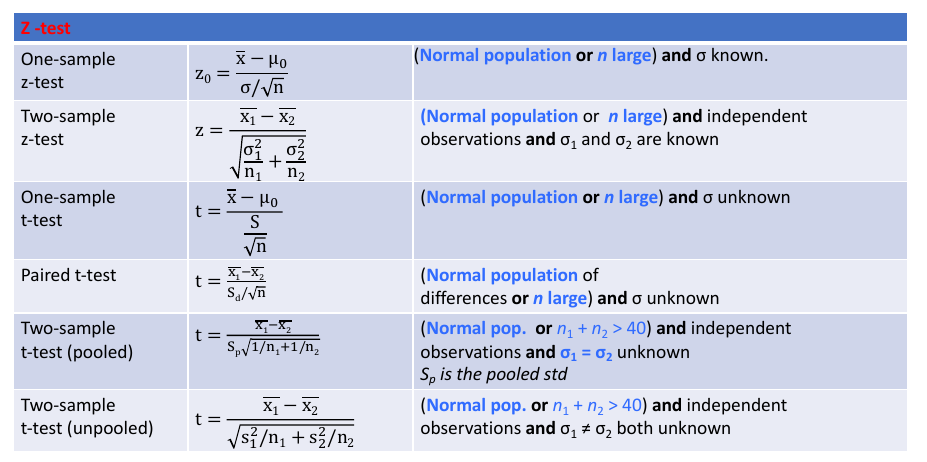
\includegraphics[width=.9\textwidth]{img/chapter-4/test-situations.png}
\caption{Tabella di scelta della tipologia di test}\label{img:test-situation}
\end{figure}

\clearpage
\subsection{Esempio di utilizzo dello Z-test}
Considera di essere un data analyst per la tua compagnia, e di dover valutare il \textbf{tempo di risposta}, che è la chiave del servizio, dato il \textbf{nuovo rilascio del software}. Si vuole quindi comparare se il nuovo update ha \textbf{cambiato significativamente} la response time rispetto al \textbf{sistema precedente}.

\subsubsection{Verifica delle assunzioni}
Nel nostro caso:
\begin{itemize}
    \item \textbf{Data (nel nostro caso la media campionaria)}: segue una distribuzione normale (ciò ci viene garantito dal fatto che si avrà una sample size molto grande e che quindi, applicando il teorema del limire centrale, si potrà dire che i dati seguono una normale)
    \item \textbf{La deviazione standard}: si conosce in maniera approssimativa andandola a calcolare mediante la \textbf{sample standard Deviation}, che è una buona stima della deviazione standard della popolazione data la grande dimensione del campione
    \item \textbf{Independent samples}: Ogni misurazione fatta della response time non è dipendente in alcun modo dalle altre
\end{itemize}

\subsubsection{Definire le ipotesi}
La definizione delle ipotesi è la seguente:
\begin{itemize}
    \item \(H_0\): l'aggiornamento non ha alcun effetto sul response time (le medie sono uguali):
    \[
    H_0: \mu_{before} = \mu_{after}
    \]

    \item \(H_1\): l'aggiornamento ha ridotto il response time, quindi:
    \[
    H_1: \mu_{before} > \mu_{after}
    \]

\end{itemize}

\subsubsection{Valutazione dei dati}
Vado a valutare, a partire dai dati a disposizione, i seguenti parametri:
\begin{itemize}
    \item \textbf{Sample Size Before Update}(\(n_{before}\)): 100
    \item \textbf{Sample Size after Update}(\(n_{after}\)): 100
    \item \textbf{Mean Response Time Before Update} (\(\overline{X}_{before}\)): 130 ms
    \item \textbf{Mean Response Time After Update} (\(\overline{X}_{after}\)): 110 ms
    \item \textbf{Sample Standard Deviation Before Update}(\(s_{before}\)): 15 ms
    \item \textbf{Sample Standard Deviation After Update}(\(s_{after}\)): 12 ms
\end{itemize}

\subsubsection{Effettuazione dello Z-test}
Dato che si vuole effettuare il \textbf{two-sample z-test}, che ha come sua formula la seguente:
\[
z = \frac{\overline{x}_1 - \overline{x}_2}{\sqrt{\frac{\sigma_1^2}{n_1} + \frac{\sigma_2^2}{n_2}}}
\]
Andando a valutare la deviazione standard, si ottiene anche lo \textbf{standard error}, che è possibile calcolare come:
\[
SE = \sqrt{\frac{\sigma_1^2}{n_1} + \frac{\sigma_2^2}{n_2}} = \sqrt{\frac{s_{before}^2}{n_{before}} + \frac{s_{after}^2}{n_{after}}} = \sqrt{\frac{15^2}{100} + \frac{12^2}{100}} = \sqrt{3.69} \approx 1.92
\]

Calcolato lo standard error vado a valutare la Z-statistic, come:
\[
z = \frac{\overline{X}_{before} - \overline{X}_{after}}{SE} = \frac{130 - 110}{1.92} \approx 10.42
\]

Una volta valutata la statistica, si vanno a valutare i valori critici e la regione critica. Per fare ciò si parte dal prefissare un \textbf{livello di confidenza}, per l'esempio si sceglierà del \(5\%\) (\(\alpha = 0.05\)). Dato che nel nostro caso siamo in una one-tailed test (consideriamo solo une delle due code, da come è impostata l'ipotesi), allora si va a calcolare il valore critico come:
\[
Z_\alpha = 1.645
\]
(\textit{Tale valore è stato prelevato da una tabella specifica})
\\
Ma, dato che la z-statistic è \(10.42\), che è maggiore di \(1.645\), allora si va a rifiutare l'ipotesi nulla.

\subsubsection{Conclusion}
Alla fine il risultato ci suggerisce che l'aggiornamento che è stato effettuato al software ha ridotto in maniera significativa il response time, supportando l'ipotesi che la nuova versione ha portato ad un incremento delle performance.

\begin{figure}[h]
\centering
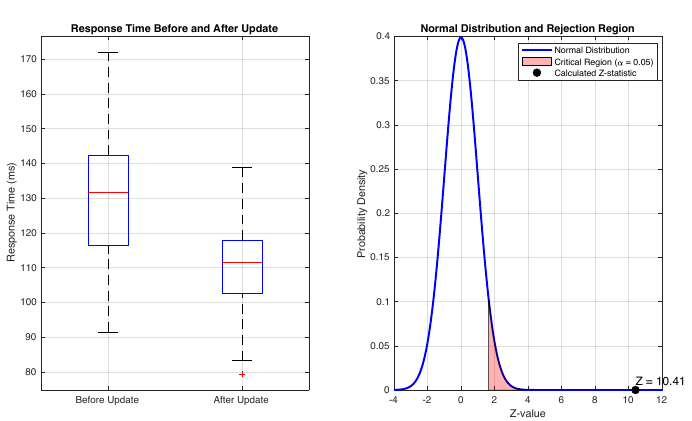
\includegraphics[width=.6\textwidth]{img/chapter-4/esempio-z-test.png}
\caption{Grafici e boxplots associati all'esempio svolto}
\end{figure}